\section{PS7: Kronos Log Parsing}\label{sec:ps7}

\subsection{Discussion}\label{sec:ps7:disc}

This project calls a log file from a Kronos InTouch time clock by using regex library expressions and makes a .rpt file to leave new logs with the time by using boost date time libraries.

\begin{figure}[tbh]
	\centering
	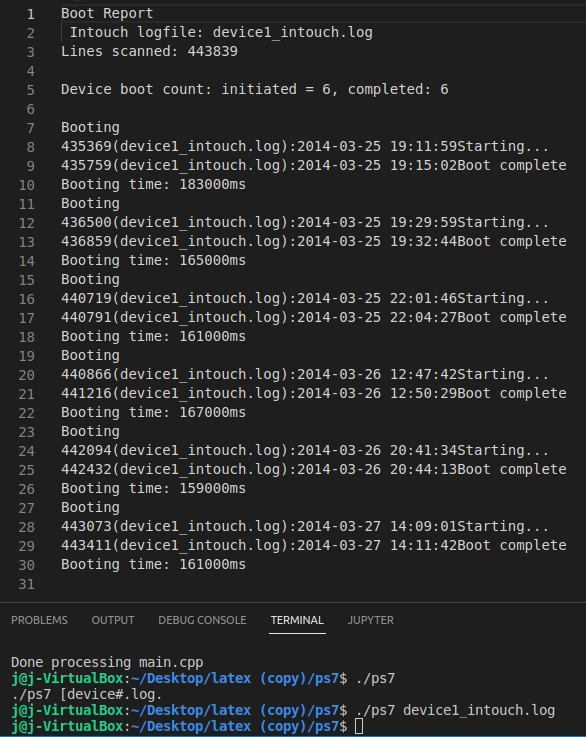
\includegraphics[width=8cm]{ps7}
	\caption{Output .rpt file}
	\label{fig:ps7}
\end{figure}

I declared using since for the date functions, there is a lot of things follow with it and stackoverflow suggested me to use it. For regex, it is not long as date, so I did not use using.

I used regular expressions to find matching string from the log file.
boost::regex-match or boost::regex-search were used to find a match against the regular expressions previously created.

\subsection{Places to get help}
I got help from Regex lecture slide, stackoverflow, c++.com

%\subsection{What I accomplished}\label{sec:ps0:accomplish}

%\subsection{What I already knew}\label{sec:ps0:knew}

%\subsection{What I learned}\label{sec:ps0:learned}

\subsection{Challenges}\label{sec:ps7:challenges}
The string for regex was a struggle due to the typo I spend too much time finding out my mistake.

\subsection{Mistakes}\label{sec:ps7:Mistakes}

I got two points off because my formatting had problem, and did not describe regexes in readme.

\subsection{Extra Credit}\label{sec:ps7:Extra Credit}

I got 0.5 extra credit because my program had header but not mentioned in readme.

\subsection{Codebase}\label{sec:ps7:code}
Makefile
\lstinputlisting[language=Make]{ps7/Makefile}
main.cpp
\lstinputlisting{ps7/main.cpp}

\newpage
